\chapter{演员-评论家方法}
\label{ch:rl-ac}

% ════════════════════════════════════════════════════════════════
%  忠实转录自《强化学习的数学原理》(赵世钰) 第10章「演员-评论家方法」。
%  以源页 PDF (p233--p254) 为完整性与正确性基准，逐公式对照纠正 OCR。
%  本章为新部「强化学习理论」(P6_rl) 的一章。
% ════════════════════════════════════════════════════════════════

% TODO[图10.1]：Zhao「本章在全书中的位置」导航图，按约定弃用。
%   源图 images/9b8ca7a170d64faec3b4312c9d1b00333f69aa24b0d8e7ad4afe39190fd793cb.jpg
%   注：源书图10.1=被弃用的导航图，故本章正文用 \cref 引用的重要性采样图在
%   源页编号为「图10.2」。下面 figure 环境内 \addtocounter{figure}{1} 占位，使其
%   自动编号对齐源页「图10.2」（本部各章按既定弃图约定统一处理）。

本章将介绍 Actor-Critic 方法，该方法的中文翻译一般为“演员-评论家”。从一个角度来看，Actor-Critic 指的是一种结构，它融合了基于策略和基于价值的两类方法。这里的“Actor”对应的是策略更新。之所以称之为 Actor，是因为它对应生成动作的策略。这里的“Critic”指的是价值更新。之所以称之为 Critic，是因为它会评估策略相应的价值。从另一个角度看，Actor-Critic 本质上仍然是策略梯度的方法，它可以通过推广第 9 章介绍的策略梯度方法得到。在学习本章之前，读者应该确保已经比较好地了解了第 8 章和第 9 章的内容，否则学习本章时会遇到诸多挑战。

% ════════════════════════════════════════════════════════════════
\section{最简单的演员-评论家算法：QAC}
\label{sec:rl-ac-qac}

本节将介绍最简单的 Actor-Critic 算法。我们可以通过推广式~\eqref{eq:rl-ac-pg-grad} 中的策略梯度算法很容易地得到该算法。

首先，让我们回想一下。策略梯度方法的基本思想是通过最大化一个目标函数 $J(\theta)$ 来得到最优策略。用于最大化 $J(\theta)$ 的梯度上升算法是
\begin{equation}
\begin{aligned}
\theta_{t+1} &= \theta_{t} + \alpha \nabla_{\theta} J(\theta_{t}) \\
&= \theta_{t} + \alpha \mathbb{E}_{S \sim \eta, A \sim \pi} \Big[ \nabla_{\theta} \ln \pi(A | S, \theta_{t}) q_{\pi}(S, A) \Big],
\end{aligned}
\label{eq:rl-ac-pg-grad}
\end{equation}
其中 $\eta$ 是状态的分布（更多信息可参见定理~9.1）。由于真实的梯度是无法得到的，我们可以使用随机梯度来近似：
\begin{equation}
\theta_{t+1} = \theta_{t} + \alpha \nabla_{\theta} \ln \pi(a_{t} | s_{t}, \theta_{t}) q_{t}(s_{t}, a_{t}).
\label{eq:rl-ac-sgd}
\end{equation}
这就是上一章式 (9.32) 中给出的算法。

式~\eqref{eq:rl-ac-sgd} 非常重要，因为它清楚地展示了如何融合基于策略的方法和基于价值的方法。一方面，它是一个基于策略的算法，因为它直接更新策略参数。另一方面，它的更新需要知道 $q_{t}(s_{t}, a_{t})$，这是动作值 $q_{\pi}(s_{t}, a_{t})$ 的估计量，需要另一个基于价值的算法来得到 $q_{t}(s_{t}, a_{t})$。

到目前为止，本书介绍了两种估计动作值的方法：第一种是基于蒙特卡罗的方法，第二种是时序差分的方法。

如果 $q_{t}(s_{t}, a_{t})$ 是通过蒙特卡罗方法来估计的，那么相应的算法被称为 REINFORCE 或者蒙特卡罗策略梯度。该算法已经在第 9 章介绍过了。

如果 $q_{t}(s_{t}, a_{t})$ 是通过时序差分方法来估计的，那么相应的算法通常被称为 Actor-Critic。换句话说，当我们把基于时序差分的价值估计引入到策略梯度方法时，就得到了 Actor-Critic 方法。

算法~\ref{alg:rl-ac-qac} 给出了最简单的 Actor-Critic 算法。其中 Actor 对应于式~\eqref{eq:rl-ac-sgd} 给出的策略更新步骤；Critic 对应于式 (8.36) 给出的 Sarsa 算法，用于估计策略对应的值，其中动作值由函数 $q(s, a, w)$ 表示。这种 Actor-Critic 算法有时被称为 Q Actor-Critic（QAC）。尽管它很简单，但 QAC 揭示了 Actor-Critic 算法的核心思想。我们在本章后面看到的许多高级算法都可以通过推广 QAC 得到。

\begin{algo}[最简单的 Actor-Critic 算法（QAC）]\label{alg:rl-ac-qac}
\textbf{初始化}：一个策略函数 $\pi(a | s, \theta_{0})$，其中 $\theta_{0}$ 是初始参数。一个值函数 $q(s, a, w_{0})$，其中 $w_{0}$ 是初始参数。$\alpha_{w}, \alpha_{\theta} > 0$。

\textbf{目标}：学习一个最优策略来最大化 $J(\theta)$。

在每个回合中的 $t$ 时刻：

\quad 根据 $\pi(a | s_{t}, \theta_{t})$ 产生 $a_{t}$，观测 $r_{t+1}, s_{t+1}$，然后根据 $\pi(a | s_{t+1}, \theta_{t})$ 生成 $a_{t+1}$。

\quad Actor（策略更新）：
\[
\theta_{t+1} = \theta_{t} + \alpha_{\theta} \nabla_{\theta} \ln \pi(a_{t} | s_{t}, \theta_{t}) q(s_{t}, a_{t}, w_{t})
\]

\quad Critic（价值更新）：
\[
w_{t+1} = w_{t} + \alpha_{w} \big[ r_{t+1} + \gamma q(s_{t+1}, a_{t+1}, w_{t}) - q(s_{t}, a_{t}, w_{t}) \big] \nabla_{w} q(s_{t}, a_{t}, w_{t})
\]
\end{algo}

% ════════════════════════════════════════════════════════════════
\section{优势演员-评论家}
\label{sec:rl-ac-a2c}

下面介绍优势演员-评论家（advantage actor-critic，A2C）算法。这个算法的核心思想是引入一个基准来减少估计的方差。

\subsection{基准不变性}
\label{sec:rl-ac-baseline}

策略梯度有一个重要性质：它对额外的基准（baseline）是不变的，即
\begin{equation}
\mathbb{E}_{S \sim \eta, A \sim \pi} \Big[ \nabla_{\theta} \ln \pi(A | S, \theta_{t}) q_{\pi}(S, A) \Big]
= \mathbb{E}_{S \sim \eta, A \sim \pi} \Big[ \nabla_{\theta} \ln \pi(A | S, \theta_{t}) \big( q_{\pi}(S, A) - b(S) \big) \Big],
\label{eq:rl-ac-baseline-inv}
\end{equation}
其中 $b(S)$ 是基准函数，它是 $S$ 的一个标量函数。上式表明了添加或去掉基准函数 $b(S)$ 不会影响策略梯度。下面回答两个重要问题。

\paragraph{第一，为什么式~\eqref{eq:rl-ac-baseline-inv} 是成立的？}
式~\eqref{eq:rl-ac-baseline-inv} 成立的充分必要条件是下式成立：
\[
\mathbb{E}_{S \sim \eta, A \sim \pi} \Big[ \nabla_{\theta} \ln \pi(A | S, \theta_{t}) b(S) \Big] = 0.
\]
而该式成立的原因如下所示：
\[
\begin{aligned}
\mathbb{E}_{S \sim \eta, A \sim \pi} \Big[ \nabla_{\theta} \ln \pi(A | S, \theta_{t}) b(S) \Big]
&= \sum_{s \in \mathcal{S}} \eta(s) \sum_{a \in \mathcal{A}} \pi(a | s, \theta_{t}) \nabla_{\theta} \ln \pi(a | s, \theta_{t}) b(s) \\
&= \sum_{s \in \mathcal{S}} \eta(s) \sum_{a \in \mathcal{A}} \nabla_{\theta} \pi(a | s, \theta_{t}) b(s) \\
&= \sum_{s \in \mathcal{S}} \eta(s) b(s) \sum_{a \in \mathcal{A}} \nabla_{\theta} \pi(a | s, \theta_{t}) \\
&= \sum_{s \in \mathcal{S}} \eta(s) b(s) \nabla_{\theta} \sum_{a \in \mathcal{A}} \pi(a | s, \theta_{t}) \\
&= \sum_{s \in \mathcal{S}} \eta(s) b(s) \nabla_{\theta} 1 = 0.
\end{aligned}
\]

\paragraph{第二，为什么我们要引入基准函数？它有什么用？}
基准函数之所以有用，是因为它能够在我们使用随机样本近似真实梯度时减少近似的方差。具体来说，定义
\begin{equation}
X(S, A) \doteq \nabla_{\theta} \ln \pi(A | S, \theta_{t}) \big[ q_{\pi}(S, A) - b(S) \big].
\label{eq:rl-ac-X}
\end{equation}
此时真实的梯度是 $\mathbb{E}[X(S, A)]$。由于我们需要使用一个随机样本 $x$ 来近似 $\mathbb{E}[X]$ 的值，我们希望方差 $\operatorname{var}(X)$ 越小越好。如果 $\operatorname{var}(X)$ 接近 0，那么任何样本 $x$ 都可以准确地近似 $\mathbb{E}[X]$。相反，如果 $\operatorname{var}(X)$ 很大，样本 $x$ 的值可能和 $\mathbb{E}[X]$ 有较大差距，此时用 $x$ 来近似 $\mathbb{E}[X]$ 可能很不准确。

虽然 $\mathbb{E}[X]$ 对于基准是不变的，但是方差 $\operatorname{var}(X)$ 是会随着基准变化的。因此，我们可以设计一个好的基准从而最小化 $\operatorname{var}(X)$。在 REINFORCE 和 QAC 的算法中，我们实际上设置了 $b = 0$，而这不一定是一个好的基准函数。

事实上，能够最小化 $\operatorname{var}(X)$ 的最优基准是
\begin{equation}
b^{*}(s) = \frac{\mathbb{E}_{A \sim \pi} \big[ \| \nabla_{\theta} \ln \pi(A | s, \theta_{t}) \|^{2} q_{\pi}(s, A) \big]}{\mathbb{E}_{A \sim \pi} \big[ \| \nabla_{\theta} \ln \pi(A | s, \theta_{t}) \|^{2} \big]}, \quad s \in \mathcal{S}.
\label{eq:rl-ac-optimal-baseline}
\end{equation}
详细的证明可参见方框~\ref{box:rl-ac-optbaseline}。

尽管式~\eqref{eq:rl-ac-optimal-baseline} 中的基准是最优的，但它太复杂，无法在实际中使用。如果从式~\eqref{eq:rl-ac-optimal-baseline} 中移除权重 $\| \nabla_{\theta} \ln \pi(A | s, \theta_{t}) \|^{2}$，就可以得到一个次优的基准，它有一个简洁的表达式：
\[
b^{\dagger}(s) = \mathbb{E}_{A \sim \pi} [ q_{\pi}(s, A) ] = v_{\pi}(s), \quad s \in \mathcal{S}.
\]
值得注意的是，这个次优的基准函数就是状态值函数。

\begin{derivation}[方框 10.1：证明式~\eqref{eq:rl-ac-optimal-baseline} 中的 $b^{*}(s)$ 是最优基准]\label{box:rl-ac-optbaseline}
令 $\bar{x} \doteq \mathbb{E}[X]$。如果 $X$ 是一个向量，那么其方差 $\operatorname{var}(X)$ 是一个矩阵。通常可以选择其迹（trace）作为优化的标量目标函数：
\begin{equation}
\begin{aligned}
\operatorname{tr}[\operatorname{var}(X)] &= \operatorname{tr} \mathbb{E}[(X - \bar{x})(X - \bar{x})^{\mathrm{T}}] \\
&= \operatorname{tr} \mathbb{E}[X X^{\mathrm{T}} - \bar{x} X^{\mathrm{T}} - X \bar{x}^{\mathrm{T}} + \bar{x} \bar{x}^{\mathrm{T}}] \\
&= \mathbb{E}[X^{\mathrm{T}} X - X^{\mathrm{T}} \bar{x} - \bar{x}^{\mathrm{T}} X + \bar{x}^{\mathrm{T}} \bar{x}] \\
&= \mathbb{E}[X^{\mathrm{T}} X] - \bar{x}^{\mathrm{T}} \bar{x}.
\end{aligned}
\label{eq:rl-ac-trvar}
\end{equation}
在导出上式时，我们使用了迹的性质 $\operatorname{tr}(AB) = \operatorname{tr}(BA)$，其中 $A, B$ 是两个方阵。如果 $\bar{x}$ 是不变的，那么式~\eqref{eq:rl-ac-trvar} 表明我们只需要最小化 $\mathbb{E}[X^{\mathrm{T}} X]$ 就可以最小化 $\operatorname{tr}[\operatorname{var}(X)]$。

把 $X$ 在式~\eqref{eq:rl-ac-X} 中的表达式代入 $\mathbb{E}[X^{\mathrm{T}} X]$ 可得
\[
\begin{aligned}
\mathbb{E}[X^{\mathrm{T}} X] &= \mathbb{E} \left[ (\nabla_{\theta} \ln \pi)^{\mathrm{T}} (\nabla_{\theta} \ln \pi) (q_{\pi}(S, A) - b(S))^{2} \right] \\
&= \mathbb{E} \left[ \| \nabla_{\theta} \ln \pi \|^{2} (q_{\pi}(S, A) - b(S))^{2} \right],
\end{aligned}
\]
其中 $\pi(A | S, \theta)$ 简写为 $\pi$。由于 $S \sim \eta$ 且 $A \sim \pi$，上述方程可以改写为
\[
\mathbb{E}[X^{\mathrm{T}} X] = \sum_{s \in \mathcal{S}} \eta(s) \mathbb{E}_{A \sim \pi} \left[ \| \nabla_{\theta} \ln \pi \|^{2} (q_{\pi}(s, A) - b(s))^{2} \right].
\]
目标函数最优的必要条件是 $\nabla_{b} \mathbb{E}[X^{\mathrm{T}} X] = 0$。为确保 $\nabla_{b} \mathbb{E}[X^{\mathrm{T}} X] = 0$，对任意 $s \in \mathcal{S}$，$b(s)$ 应满足
\[
\mathbb{E}_{A \sim \pi} \big[ \| \nabla_{\theta} \ln \pi \|^{2} (b(s) - q_{\pi}(s, A)) \big] = 0.
\]
不难求解上述方程进而得到最优基准函数：
\[
b^{*}(s) = \frac{\mathbb{E}_{A \sim \pi} [ \| \nabla_{\theta} \ln \pi \|^{2} q_{\pi}(s, A) ]}{\mathbb{E}_{A \sim \pi} [ \| \nabla_{\theta} \ln \pi \|^{2} ]}, \qquad s \in \mathcal{S}.
\]
关于策略梯度方法中最优基准的更多讨论可参见 [69, 70]。
\end{derivation}

\subsection{算法描述}
\label{sec:rl-ac-a2c-alg}

当 $b(s) = v_{\pi}(s)$ 时，式~\eqref{eq:rl-ac-pg-grad} 中的梯度上升算法变成了
\begin{equation}
\begin{aligned}
\theta_{t+1} &= \theta_{t} + \alpha \mathbb{E} \Big[ \nabla_{\theta} \ln \pi(A | S, \theta_{t}) [ q_{\pi}(S, A) - v_{\pi}(S) ] \Big] \\
&\doteq \theta_{t} + \alpha \mathbb{E} \Big[ \nabla_{\theta} \ln \pi(A | S, \theta_{t}) \delta_{\pi}(S, A) \Big],
\end{aligned}
\label{eq:rl-ac-a2c-grad}
\end{equation}
其中
\[
\delta_{\pi}(S, A) \doteq q_{\pi}(S, A) - v_{\pi}(S)
\]
被称为优势函数（advantage function），它反映了一个动作相对于其他动作的优势。具体来说，由于状态值 $v_{\pi}(s) = \sum_{a \in \mathcal{A}} \pi(a | s) q_{\pi}(s, a)$ 是平均动作值，因此 $\delta_{\pi}(s, a) > 0$ 意味着相应的动作值大于均值，具有一定的优势。

如果把式~\eqref{eq:rl-ac-a2c-grad} 中的真实梯度替换成随机梯度，可以得到
\begin{equation}
\begin{aligned}
\theta_{t+1} &= \theta_{t} + \alpha \nabla_{\theta} \ln \pi(a_{t} | s_{t}, \theta_{t}) [ q_{t}(s_{t}, a_{t}) - v_{t}(s_{t}) ] \\
&= \theta_{t} + \alpha \nabla_{\theta} \ln \pi(a_{t} | s_{t}, \theta_{t}) \delta_{t}(s_{t}, a_{t}).
\end{aligned}
\label{eq:rl-ac-a2c-sgd}
\end{equation}
其中 $s_{t}, a_{t}$ 是在 $t$ 时刻 $S, A$ 的样本。这里 $q_{t}(s_{t}, a_{t})$ 和 $v_{t}(s_{t})$ 分别是 $q_{\pi(\theta_{t})}(s_{t}, a_{t})$ 和 $v_{\pi(\theta_{t})}(s_{t})$ 的估计值。值得指出的是，算法~\eqref{eq:rl-ac-a2c-sgd} 是基于 $q_{t} - v_{t}$ 这个相对值更新策略的，而不是基于其绝对值。这在直观上是合理的，因为当我们在一个状态选择一个动作时，我们只关心哪个动作相对于其他动作具有更大的价值，而并不关心其绝对动作值。

如果 $q_{t}(s_{t}, a_{t})$ 和 $v_{t}(s_{t})$ 是通过蒙特卡罗方法估计的，那么式~\eqref{eq:rl-ac-a2c-sgd} 中的算法被称为带基准的 REINFORCE（REINFORCE with baseline）。如果 $q_{t}(s_{t}, a_{t})$ 和 $v_{t}(s_{t})$ 是通过时序差分方法估计的，那么这种算法通常被称为 Advantage Actor-Critic（A2C）。算法~\ref{alg:rl-ac-a2c} 给出了 A2C 算法的流程。应该注意的是，算法~\ref{alg:rl-ac-a2c} 中的优势函数是通过时序差分误差近似的，即
\[
q_{t}(s_{t}, a_{t}) - v_{t}(s_{t}) \approx r_{t+1} + \gamma v_{t}(s_{t+1}) - v_{t}(s_{t}).
\]
这个近似是合理的原因是
\[
q_{\pi}(s_{t}, a_{t}) - v_{\pi}(s_{t}) = \mathbb{E} \Big[ R_{t+1} + \gamma v_{\pi}(S_{t+1}) - v_{\pi}(S_{t}) \,\big|\, S_{t} = s_{t}, A_{t} = a_{t} \Big].
\]
上式是基于 $q_{\pi}(s_{t}, a_{t})$ 的原始定义得到的。使用时序差分误差的一个优势是我们只需要使用一个神经网络来表征 $v_{\pi}(s)$。相反，如果我们使用 $\delta_{t} = q_{t}(s_{t}, a_{t}) - v_{t}(s_{t})$，则需要维护两个网络来分别表示 $v_{\pi}(s)$ 和 $q_{\pi}(s, a)$。当我们使用时序差分误差时，该算法也被称为 TD Actor-Critic。此外，值得注意的是，$\pi(\theta_{t})$ 是一个随机策略，因此它具有一定的探索性，所以它可以直接用来生成经验样本，而不需要诸如 $\epsilon$-Greedy 之类的技巧。A2C 还有一些变体，例如 A3C（asynchronous advantage actor-critic）等。感兴趣的读者可以参考文献 [71, 72]。

\begin{algo}[Advantage Actor-Critic（A2C）或 TD Actor-Critic]\label{alg:rl-ac-a2c}
\textbf{初始化}：策略函数 $\pi(a | s, \theta_{0})$，其中 $\theta_{0}$ 是初始参数。值函数 $v(s, w_{0})$，其中 $w_{0}$ 是初始参数。$\alpha_{w}, \alpha_{\theta} > 0$。

\textbf{目标}：学习最优策略以最大化 $J(\theta)$。

在每个回合中的 $t$ 时刻：

\quad 根据 $\pi(a | s_{t}, \theta_{t})$ 生成 $a_{t}$，然后得到 $r_{t+1}, s_{t+1}$。

\quad 优势函数（时序差分误差）：
\[
\delta_{t} = r_{t+1} + \gamma v(s_{t+1}, w_{t}) - v(s_{t}, w_{t})
\]

\quad Actor（策略更新）：
\[
\theta_{t+1} = \theta_{t} + \alpha_{\theta} \delta_{t} \nabla_{\theta} \ln \pi(a_{t} | s_{t}, \theta_{t})
\]

\quad Critic（价值更新）：
\[
w_{t+1} = w_{t} + \alpha_{w} \delta_{t} \nabla_{w} v(s_{t}, w_{t})
\]
\end{algo}

% ════════════════════════════════════════════════════════════════
\section{异策略演员-评论家}
\label{sec:rl-ac-offpolicy}

迄今为止，我们介绍的策略梯度方法，包括 REINFORCE、QAC、A2C 都是同策略（on-policy）的，其原因可以从真实梯度的表达式中看出：
\[
\nabla_{\theta} J(\theta) = \mathbb{E}_{S \sim \eta, A \sim \pi} \Big[ \nabla_{\theta} \ln \pi(A | S, \theta_{t}) \big( q_{\pi}(S, A) - v_{\pi}(S) \big) \Big].
\]
为了使用随机梯度来近似这个真实梯度，我们必须按照 $\pi(\theta)$ 生成动作样本。因此，$\pi(\theta)$ 是行为策略。因为 $\pi(\theta)$ 也是我们要改进的目标策略，所以策略梯度方法是 On-policy 的。

如果我们已经有一些由其他行为策略生成的样本，那么策略梯度方法仍然可以使用这些样本来得到最优策略，此时的方法就变成了异策略（off-policy），不过此时需要采用一种称为重要性采样（importance sampling）的技术。值得一提的是，重要性采样并不仅限于强化学习领域，它是通过使用根据某一个概率分布得到的样本来估计另一个概率分布的期望值的一种通用技术。

\subsection{重要性采样}
\label{sec:rl-ac-is}

考虑一个随机变量 $X \in \mathcal{X}$。假设 $p_{0}(X)$ 是一个概率分布，我们的目标是估计 $\mathbb{E}_{X \sim p_{0}}[X]$。假设我们有一些独立同分布的样本 $\{x_{i}\}_{i=1}^{n}$。

\paragraph{第一个场景：}样本 $\{x_{i}\}_{i=1}^{n}$ 是根据 $p_{0}$ 生成的。此时，平均值 $\bar{x} = \frac{1}{n} \sum_{i=1}^{n} x_{i}$ 可以用来近似 $\mathbb{E}_{X \sim p_{0}}[X]$。这是因为 $\bar{x}$ 是 $\mathbb{E}_{X \sim p_{0}}[X]$ 的无偏估计，并且估计的方差随着 $n \to \infty$ 收敛到 0。更多信息请参见方框 5.1 中的大数定律。

\paragraph{第二个场景：}样本 $\{x_{i}\}_{i=1}^{n}$ 不是根据 $p_{0}$ 生成的，而是根据另一个概率分布 $p_{1}$ 生成的。我们是否仍然可以使用这些样本来近似 $\mathbb{E}_{X \sim p_{0}}[X]$ 呢？答案是可以的。然而，我们不能再使用 $\bar{x} = \frac{1}{n} \sum_{i=1}^{n} x_{i}$ 来近似 $\mathbb{E}_{X \sim p_{0}}[X]$，这是因为 $\bar{x} \approx \mathbb{E}_{X \sim p_{1}}[X]$ 而非 $\mathbb{E}_{X \sim p_{0}}[X]$。

在第二个场景中，我们就需要使用重要性采样的技术来估计 $\mathbb{E}_{X \sim p_{0}}[X]$。具体来说，$\mathbb{E}_{X \sim p_{0}}[X]$ 满足下式：
\begin{equation}
\mathbb{E}_{X \sim p_{0}}[X] = \sum_{x \in \mathcal{X}} p_{0}(x) x = \sum_{x \in \mathcal{X}} p_{1}(x) \underbrace{\frac{p_{0}(x)}{p_{1}(x)} x}_{f(x)} = \mathbb{E}_{X \sim p_{1}}[f(X)].
\label{eq:rl-ac-is1}
\end{equation}
上式表明，估计 $\mathbb{E}_{X \sim p_{0}}[X]$ 被转换为估计 $\mathbb{E}_{X \sim p_{1}}[f(X)]$ 的问题。此时，令
\[
\bar{f} \doteq \frac{1}{n} \sum_{i=1}^{n} f(x_{i}).
\]
因为 $\bar{f}$ 可以有效地近似 $\mathbb{E}_{X \sim p_{1}}[f(X)]$，所以由式~\eqref{eq:rl-ac-is1} 可知
\begin{equation}
\mathbb{E}_{X \sim p_{0}}[X] = \mathbb{E}_{X \sim p_{1}}[f(X)] \approx \bar{f} = \frac{1}{n} \sum_{i=1}^{n} f(x_{i}) = \frac{1}{n} \sum_{i=1}^{n} \underbrace{\frac{p_{0}(x_{i})}{p_{1}(x_{i})}}_{\text{重要性权重}} x_{i}.
\label{eq:rl-ac-is2}
\end{equation}
式~\eqref{eq:rl-ac-is2} 表明 $\mathbb{E}_{X \sim p_{0}}[X]$ 可以通过 $x_{i}$ 的加权平均来近似，而这里的权重就是 $\frac{p_{0}(x_{i})}{p_{1}(x_{i})}$，它被称为重要性权重（importance weight）。当 $p_{1} = p_{0}$ 时，重要性权重等于 1，$\bar{f}$ 就变成了 $\bar{x}$。当 $p_{0}(x_{i}) \geqslant p_{1}(x_{i})$ 时，这意味着 $x_{i}$ 可以在 $p_{0}$ 下更频繁地被采样到，而在 $p_{1}$ 下较少地被采样到。此时重要性权重大于 1，突出了这个样本的重要性。

一些读者可能会提出下面的问题：为了计算 $\mathbb{E}_{X \sim p_{0}}[X]$，式~\eqref{eq:rl-ac-is2} 需要知道 $p_{0}(x)$；如果我们已经知道了 $p_{0}(x)$，为什么不直接使用期望值的定义 $\mathbb{E}_{X \sim p_{0}}[X] = \sum_{x \in \mathcal{X}} p_{0}(x) x$ 来计算呢？这个问题具有一定的迷惑性。答案如下所述。实际上，如果要使用定义来计算 $\mathbb{E}_{X \sim p_{0}}[X]$，我们需要知道 $p_{0}$ 的解析表达式或者对于每一个 $x \in \mathcal{X}$ 的 $p_{0}(x)$ 的值。然而，当分布是由一个神经网络表示时，我们难以获得 $p_{0}$ 的解析表达式；或者当 $\mathcal{X}$ 很大时，也难以获得对于每一个 $x \in \mathcal{X}$ 的 $p_{0}(x)$ 的值。相比之下，式~\eqref{eq:rl-ac-is2} 仅需要一些样本的 $p_{0}(x_{i})$ 的值，因此在实践中更容易实施。

下面来看一个例子，从而更好地理解重要性采样。

\begin{example}[重要性采样的演示]\label{ex:rl-ac-is}
考虑 $X \in \mathcal{X} \doteq \{+1, -1\}$，即每次采样只能得到 $+1$ 或者 $-1$ 的样本。假设一个概率分布 $p_{0}$ 满足
\[
p_{0}(X = +1) = 0.5, \quad p_{0}(X = -1) = 0.5.
\]
根据期望值的定义，我们知道 $X$ 在 $p_{0}$ 上的真实期望值是
\[
\mathbb{E}_{X \sim p_{0}}[X] = (+1) \cdot 0.5 + (-1) \cdot 0.5 = 0.
\]
假设另一个概率分布 $p_{1}$ 满足
\[
p_{1}(X = +1) = 0.8, \quad p_{1}(X = -1) = 0.2.
\]
根据期望值的定义，我们知道 $X$ 在 $p_{1}$ 上的真实期望值是
\[
\mathbb{E}_{X \sim p_{1}}[X] = (+1) \cdot 0.8 + (-1) \cdot 0.2 = 0.6.
\]
假设我们有一些样本 $\{x_{i}\}$，这些样本是根据 $p_{1}$ 采样得到的，此时我们的任务是利用这些样本来估计 $\mathbb{E}_{X \sim p_{0}}[X]$。\cref{fig:rl-ac-is} 展示了采集到的样本，其中 $+1$ 的样本数量远多于 $-1$，这是因为 $p_{1}(X = +1) = 0.8 > p_{1}(X = -1) = 0.2$。此时如果我们直接计算样本的平均值，那么这个值会收敛到 $\mathbb{E}_{X \sim p_{1}}[X] = 0.6$（见 \cref{fig:rl-ac-is} 中的虚线）。如果我们利用式~\eqref{eq:rl-ac-is2} 计算加权平均值，那么这个值可以成功地收敛到 $\mathbb{E}_{X \sim p_{0}}[X] = 0$（见 \cref{fig:rl-ac-is} 中的实线）。
\end{example}

\begin{figure}[ht]
\centering
\addtocounter{figure}{1}% 占位被弃用的导航图10.1，使本图自动编号对齐源页「图10.2」
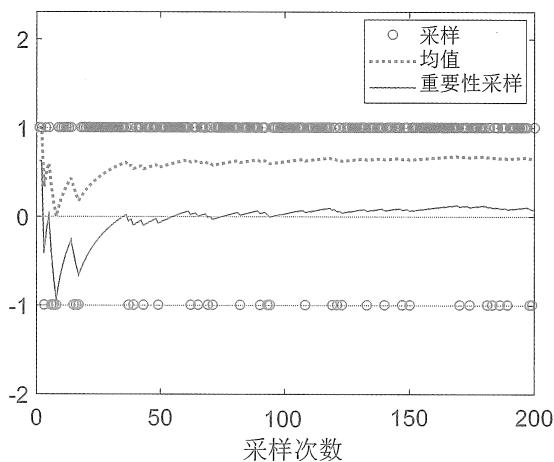
\includegraphics[width=0.78\linewidth]{figures/rl/8fab5bd32f854e1c475db326607ca56a846195d86c5a34d50d38d344ab710418.jpg}
\caption{用于演示重要性采样的例子。这里 $X \in \{+1, -1\}$ 且 $p_{0}(X = +1) = p_{0}(X = -1) = 0.5$。样本根据 $p_{1}$ 生成，其中 $p_{1}(X = +1) = 0.8$ 且 $p_{1}(X = -1) = 0.2$。样本的平均值收敛于 $\mathbb{E}_{X \sim p_{1}}[X] = 0.6$，但是式~\eqref{eq:rl-ac-is2} 计算的加权平均值成功收敛于 $\mathbb{E}_{X \sim p_{0}}[X] = 0$。}
\label{fig:rl-ac-is}
\end{figure}

最后值得指出的是，由于式~\eqref{eq:rl-ac-is2} 中 $p_{1}(x)$ 位于分母，因此用于生成样本的分布 $p_{1}$ 必须满足当 $p_{0}(x) \neq 0$ 时 $p_{1}(x) \neq 0$。否则，如果 $p_{1}(x) = 0$ 而 $p_{0}(x) \neq 0$，估计结果可能会有问题。例如，假设
\[
p_{1}(X = +1) = 1, \quad p_{1}(X = -1) = 0,
\]
此时根据 $p_{1}$ 生成的样本只可能是 $+1$：$\{x_{i}\} = \{+1, +1, \ldots, +1\}$。显然，这些样本无法正确估计 $\mathbb{E}_{X \sim p_{0}}[X] = 0$，因为无论 $n$ 有多大都会有
\[
\frac{1}{n} \sum_{i=1}^{n} \frac{p_{0}(x_{i})}{p_{1}(x_{i})} x_{i} = \frac{1}{n} \sum_{i=1}^{n} \frac{p_{0}(+1)}{p_{1}(+1)} 1 = \frac{1}{n} \sum_{i=1}^{n} \frac{0.5}{1} 1 \equiv 0.5.
\]

\subsection{Off-policy 策略梯度定理}
\label{sec:rl-ac-offpg-theorem}

利用重要性采样，我们可以推导出 Off-policy 策略梯度定理。假设 $\beta$ 是一个行为策略，我们的目标是使用由 $\beta$ 生成的样本来得到一个目标策略 $\pi$，从而最大化下面的目标函数：
\[
J(\theta) = \sum_{s \in \mathcal{S}} d_{\beta}(s) v_{\pi}(s) = \mathbb{E}_{S \sim d_{\beta}}[v_{\pi}(S)],
\]
其中 $d_{\beta}$ 是在策略 $\beta$ 下的平稳分布，$v_{\pi}$ 是在策略 $\pi$ 下的状态值。这个目标函数的梯度在下述定理中给出。

\begin{theorem}[Off-policy 策略梯度定理]\label{thm:rl-ac-offpg}
如果 $\gamma \in (0, 1)$，那么 $J(\theta)$ 的 Off-policy 梯度为
\begin{equation}
\nabla_{\theta} J(\theta) = \mathbb{E}_{S \sim \rho, A \sim \beta} \Big[ \underbrace{\frac{\pi(A | S, \theta)}{\beta(A | S)}}_{\text{重要性权重}} \nabla_{\theta} \ln \pi(A | S, \theta) q_{\pi}(S, A) \Big],
\label{eq:rl-ac-offpg}
\end{equation}
其中状态分布 $\rho$ 为
\[
\rho(s) \doteq \sum_{s' \in \mathcal{S}} d_{\beta}(s') \operatorname{Pr}_{\pi}(s | s'), \qquad s \in \mathcal{S}.
\]
这里 $\operatorname{Pr}_{\pi}(s | s') = \sum_{k=0}^{\infty} \gamma^{k} [P_{\pi}^{k}]_{s's} = \left[ (I - \gamma P_{\pi})^{-1} \right]_{s's}$ 是在策略 $\pi$ 下从 $s'$ 到 $s$ 的折扣总概率。
\end{theorem}

式~\eqref{eq:rl-ac-offpg} 中的 Off-policy 梯度与定理 9.1 中的 On-policy 梯度相似，但有两个区别。第一个区别是重要性权重，第二个区别是 $A \sim \beta$ 而不是 $A \sim \pi$，因此我们可以使用由 $\beta$ 采样得到的样本来近似真实梯度。该定理的证明在方框~\ref{box:rl-ac-offpg-proof} 中给出。

\begin{derivation}[方框 10.2：证明定理~\ref{thm:rl-ac-offpg}]\label{box:rl-ac-offpg-proof}
由于 $d_{\beta}$ 独立于 $\theta$，因此 $J(\theta)$ 的梯度满足
\begin{equation}
\nabla_{\theta} J(\theta) = \nabla_{\theta} \sum_{s \in \mathcal{S}} d_{\beta}(s) v_{\pi}(s) = \sum_{s \in \mathcal{S}} d_{\beta}(s) \nabla_{\theta} v_{\pi}(s).
\label{eq:rl-ac-offpg-p1}
\end{equation}
根据引理 9.2，$\nabla_{\theta} v_{\pi}(s)$ 的表达式为
\begin{equation}
\nabla_{\theta} v_{\pi}(s) = \sum_{s' \in \mathcal{S}} \operatorname{Pr}_{\pi}(s' | s) \sum_{a \in \mathcal{A}} \nabla_{\theta} \pi(a | s', \theta) q_{\pi}(s', a),
\label{eq:rl-ac-offpg-p2}
\end{equation}
其中 $\operatorname{Pr}_{\pi}(s' | s) \doteq \sum_{k=0}^{\infty} \gamma^{k} [P_{\pi}^{k}]_{ss'} = \left[ (I_{n} - \gamma P_{\pi})^{-1} \right]_{ss'}$。将~\eqref{eq:rl-ac-offpg-p2} 代入~\eqref{eq:rl-ac-offpg-p1} 得
\[
\begin{aligned}
\nabla_{\theta} J(\theta) &= \sum_{s \in \mathcal{S}} d_{\beta}(s) \nabla_{\theta} v_{\pi}(s) = \sum_{s \in \mathcal{S}} d_{\beta}(s) \sum_{s' \in \mathcal{S}} \operatorname{Pr}_{\pi}(s' | s) \sum_{a \in \mathcal{A}} \nabla_{\theta} \pi(a | s', \theta) q_{\pi}(s', a) \\
&= \sum_{s' \in \mathcal{S}} \left( \sum_{s \in \mathcal{S}} d_{\beta}(s) \operatorname{Pr}_{\pi}(s' | s) \right) \sum_{a \in \mathcal{A}} \nabla_{\theta} \pi(a | s', \theta) q_{\pi}(s', a) \\
&\doteq \sum_{s' \in \mathcal{S}} \rho(s') \sum_{a \in \mathcal{A}} \nabla_{\theta} \pi(a | s', \theta) q_{\pi}(s', a) \\
&= \sum_{s \in \mathcal{S}} \rho(s) \sum_{a \in \mathcal{A}} \nabla_{\theta} \pi(a | s, \theta) q_{\pi}(s, a) \qquad (\text{将 } s' \text{ 换为 } s) \\
&= \mathbb{E}_{S \sim \rho} \left[ \sum_{a \in \mathcal{A}} \nabla_{\theta} \pi(a | S, \theta) q_{\pi}(S, a) \right].
\end{aligned}
\]
利用重要性采样，上式可以转换为
\[
\begin{aligned}
\mathbb{E}_{S \sim \rho} \left[ \sum_{a \in \mathcal{A}} \nabla_{\theta} \pi(a | S, \theta) q_{\pi}(S, a) \right]
&= \mathbb{E}_{S \sim \rho} \left[ \sum_{a \in \mathcal{A}} \beta(a | S) \frac{\pi(a | S, \theta)}{\beta(a | S)} \frac{\nabla_{\theta} \pi(a | S, \theta)}{\pi(a | S, \theta)} q_{\pi}(S, a) \right] \\
&= \mathbb{E}_{S \sim \rho} \left[ \sum_{a \in \mathcal{A}} \beta(a | S) \frac{\pi(a | S, \theta)}{\beta(a | S)} \nabla_{\theta} \ln \pi(a | S, \theta) q_{\pi}(S, a) \right] \\
&= \mathbb{E}_{S \sim \rho, A \sim \beta} \left[ \frac{\pi(A | S, \theta)}{\beta(A | S)} \nabla_{\theta} \ln \pi(A | S, \theta) q_{\pi}(S, A) \right].
\end{aligned}
\]
证明完毕。上述证明类似于定理 9.1 的证明。
\end{derivation}

\subsection{算法描述}
\label{sec:rl-ac-offpolicy-alg}

基于 Off-policy 策略梯度定理，下面介绍 Off-policy Actor-Critic 算法。由于 Off-policy Actor-Critic 与 On-policy Actor-Critic 有许多共同之处，因此只重点介绍一些关键步骤。

第一，Off-policy 策略梯度对额外的基准函数 $b(s)$ 也是不变的。具体来说，因为 $\mathbb{E}\left[\frac{\pi(A | S, \theta)}{\beta(A | S)} \nabla_{\theta} \ln \pi(A | S, \theta) b(S)\right] = 0$，我们有
\[
\nabla_{\theta} J(\theta) = \mathbb{E}_{S \sim \rho, A \sim \beta} \left[ \frac{\pi(A | S, \theta)}{\beta(A | S)} \nabla_{\theta} \ln \pi(A | S, \theta) \big( q_{\pi}(S, A) - b(S) \big) \right].
\]
第二，为了降低估计方差，我们可以选择基准函数为 $b(S) = v_{\pi}(S)$。此时策略梯度为
\[
\nabla_{\theta} J(\theta) = \mathbb{E} \left[ \frac{\pi(A | S, \theta)}{\beta(A | S)} \nabla_{\theta} \ln \pi(A | S, \theta) \big( q_{\pi}(S, A) - v_{\pi}(S) \big) \right].
\]
第三，此时对应的随机梯度算法是
\[
\theta_{t+1} = \theta_{t} + \alpha_{\theta} \frac{\pi(a_{t} | s_{t}, \theta_{t})}{\beta(a_{t} | s_{t})} \nabla_{\theta} \ln \pi(a_{t} | s_{t}, \theta_{t}) \big( q_{t}(s_{t}, a_{t}) - v_{t}(s_{t}) \big),
\]
其中 $\alpha_{\theta} > 0$。第四，类似于 On-policy 的情况，优势函数 $q_{t}(s, a) - v_{t}(s)$ 可以被时序差分误差所替代，即
\[
q_{t}(s_{t}, a_{t}) - v_{t}(s_{t}) \approx r_{t+1} + \gamma v_{t}(s_{t+1}) - v_{t}(s_{t}) \doteq \delta_{t}(s_{t}, a_{t}).
\]
此时，该算法变成了
\[
\theta_{t+1} = \theta_{t} + \alpha_{\theta} \frac{\pi(a_{t} | s_{t}, \theta)}{\beta(a_{t} | s_{t})} \nabla_{\theta} \ln \pi(a_{t} | s_{t}, \theta) \delta_{t}(s_{t}, a_{t}).
\]
其具体步骤在算法~\ref{alg:rl-ac-offpolicy} 中给出。可以看出该算法与 A2C 算法相似，唯一的区别是在策略更新和值更新步骤都加入了额外的重要性权重。值得注意的是，除了策略更新之外，值更新也通过重要性采样变成了 Off-policy 的。实际上，重要性采样是一种通用技术，可以应用于诸多基于策略或基于值的算法。最后，算法~\ref{alg:rl-ac-offpolicy} 可以推广得到更多算法，例如可以引入 Eligibility trace 等 [73]。

\begin{algo}[基于重要性采样的 Off-policy Actor-Critic 算法]\label{alg:rl-ac-offpolicy}
\textbf{初始化}：给定一个行为策略 $\beta(a | s)$。一个目标策略 $\pi(a | s, \theta_{0})$，其中 $\theta_{0}$ 是初始参数。一个值函数 $v(s, w_{0})$，其中 $w_{0}$ 是初始参数。$\alpha_{w}, \alpha_{\theta} > 0$。

\textbf{目标}：学习一个最优策略以最大化 $J(\theta)$。

在每个回合中的 $t$ 时刻：

\quad 按照 $\beta(s_{t})$ 生成 $a_{t}$，然后得到 $r_{t+1}, s_{t+1}$。

\quad 优势函数（时序差分误差）：
\[
\delta_{t} = r_{t+1} + \gamma v(s_{t+1}, w_{t}) - v(s_{t}, w_{t})
\]

\quad Actor（策略更新）：
\[
\theta_{t+1} = \theta_{t} + \alpha_{\theta} \frac{\pi(a_{t} | s_{t}, \theta_{t})}{\beta(a_{t} | s_{t})} \delta_{t} \nabla_{\theta} \ln \pi(a_{t} | s_{t}, \theta_{t})
\]

\quad Critic（值更新）：
\[
w_{t+1} = w_{t} + \alpha_{w} \frac{\pi(a_{t} | s_{t}, \theta_{t})}{\beta(a_{t} | s_{t})} \delta_{t} \nabla_{w} v(s_{t}, w_{t})
\]
\end{algo}

% ════════════════════════════════════════════════════════════════
\section{确定性演员-评论家}
\label{sec:rl-ac-deterministic}

到目前为止，我们介绍的策略梯度算法都是基于随机策略的，即 $\pi(a | s, \theta) > 0$ 对每一个 $(s, a)$ 都成立。实际上，确定性策略也可以在策略梯度方法中使用。这里，“确定性”指的是对于任何一个状态，策略选择某一个动作的概率是 1，而选择其他动作的概率都是 0。

基于确定性策略的 Actor-Critic 方法被称为确定性 Actor-Critic（deterministic actor-critic）或者确定性策略梯度（deterministic policy gradient）。该方法非常重要，因为它天然就是 Off-policy 的，并且可以有效处理连续动作空间。

具体来说，之前我们一直使用 $\pi(a | s, \theta)$ 来表示一个策略，这个策略可以是随机性的或确定性的。在本节中，我们使用
\[
a = \mu(s, \theta)
\]
来专门表示一个确定性的策略。$\mu$ 是从 $\mathcal{S}$ 到 $\mathcal{A}$ 的一个映射，因此会直接输出一个动作。这与之前的 $\pi$ 不同：$\pi$ 输出的是某一个动作的概率。这种确定性策略也可以由神经网络来实现：例如输入是状态 $s$，输出是动作 $a$，参数是 $\theta$。简单起见，我们通常将 $\mu(s, \theta)$ 简写为 $\mu(s)$。

\subsection{确定性策略梯度定理}
\label{sec:rl-ac-dpg-theorem}

第 9 章介绍的策略梯度定理仅适用于随机策略。如果我们要求策略必须为确定性的，那么需要推导新的策略梯度定理。下面首先给出确定性策略梯度定理，再解释如何得到这个定理。

\begin{theorem}[确定性策略梯度定理]\label{thm:rl-ac-dpg}
$J(\theta)$ 的梯度是
\begin{equation}
\begin{aligned}
\nabla_{\theta} J(\theta) &= \sum_{s \in \mathcal{S}} \eta(s) \nabla_{\theta} \mu(s) \big( \nabla_{a} q_{\mu}(s, a) \big) \big|_{a = \mu(s)} \\
&= \mathbb{E}_{S \sim \eta} \left[ \nabla_{\theta} \mu(S) \big( \nabla_{a} q_{\mu}(S, a) \big) \big|_{a = \mu(S)} \right],
\end{aligned}
\label{eq:rl-ac-dpg}
\end{equation}
其中 $\eta$ 是状态的分布。
\end{theorem}

定理~\ref{thm:rl-ac-dpg} 实际上是后面定理~\ref{thm:rl-ac-dpg-discounted} 和定理~\ref{thm:rl-ac-dpg-undiscounted} 的汇总。由于定理~\ref{thm:rl-ac-dpg-discounted} 和定理~\ref{thm:rl-ac-dpg-undiscounted} 中的结果具有相似的形式，我们在定理~\ref{thm:rl-ac-dpg} 中以统一的方式呈现。具体的细节诸如 $J(\theta)$ 和 $\eta$ 的表达式将在定理~\ref{thm:rl-ac-dpg-discounted} 和定理~\ref{thm:rl-ac-dpg-undiscounted} 中给出。

确定性策略梯度方法是 Off-policy 的。这一点可以从式~\eqref{eq:rl-ac-dpg} 中的梯度表达式看出来。与随机策略情况不同，式~\eqref{eq:rl-ac-dpg} 所示的梯度并不涉及动作随机变量 $A$。因此，当我们使用样本来近似该真实梯度时无需动作样本，自然也就不需要关心动作样本是哪个策略产生的，所以生成样本的策略可以和目标策略不同。

另外，一些读者可能会好奇为什么 $\left( \nabla_{a} q_{\mu}(S, a) \right) |_{a = \mu(S)}$ 不能被写作 $\nabla_{a} q_{\mu}(S, \mu(S))$？这样看起来不是更简洁吗？如果我们这样做，就看不出来为什么 $q_{\mu}(S, \mu(S))$ 是变量 $a$ 的函数了。当然，我们也可以使用另一个简洁而不会引起混淆的表达式：$\nabla_{a} q_{\mu}(S, a = \mu(S))$。

在本节的剩余部分，我们将给出定理~\ref{thm:rl-ac-dpg} 的推导细节。我们会推导两个常见目标函数的梯度：第一个目标函数是平均状态值，第二个目标函数是平均奖励值。由于这两个目标函数已经在第 9.2 节详细讨论过，因此我们有时会不加说明地使用它们的一些性质。

对于大多数读者而言，只要熟悉定理~\ref{thm:rl-ac-dpg} 的结论就足够了，而并不需要了解其推导细节。对推导细节感兴趣的读者可以有选择性地阅读本节后面的内容。

\subsection*{目标函数 1：平均状态值}

我们首先推导平均状态值的梯度。平均状态值的表达式是
\begin{equation}
J(\theta) = \mathbb{E}[v_{\mu}(s)] = \sum_{s \in \mathcal{S}} d_{0}(s) v_{\mu}(s),
\label{eq:rl-ac-J-avgstate}
\end{equation}
其中 $d_{0}$ 是状态的概率分布。简单起见，我们可以假设 $d_{0}$ 是一个与策略 $\mu$ 独立的分布，这样 $d_{0}$ 对 $\theta$ 的梯度等于 0。$d_{0}$ 的选择有两种特殊但重要的情形。第一种情形是选择 $d_{0}(s_{0}) = 1$ 且 $d_{0}(s \neq s_{0}) = 0$，其中 $s_{0}$ 是一个我们感兴趣的特定状态。在这种情况下，学习到的策略旨在最大化从 $s_{0}$ 出发获得的回报。第二种情形是选择 $d_{0}$ 为一个给定的行为策略的分布，该行为策略可以与目标策略不同。

为了计算 $J(\theta)$ 的梯度，我们需要首先计算对任意状态 $s \in \mathcal{S}$ 的状态值 $v_{\mu}(s)$ 的梯度。

\begin{theorem}[$v_{\mu}(s)$ 的梯度（引理 10.1）]\label{thm:rl-ac-lemma-vmu}
当 $\gamma \in (0, 1)$，对于任意 $s \in \mathcal{S}$ 有
\begin{equation}
\nabla_{\theta} v_{\mu}(s) = \sum_{s' \in \mathcal{S}} \operatorname{Pr}_{\mu}(s' | s) \nabla_{\theta} \mu(s') \big( \nabla_{a} q_{\mu}(s', a) \big) \big|_{a = \mu(s')},
\label{eq:rl-ac-vmu-grad}
\end{equation}
其中
\[
\operatorname{Pr}_{\mu}(s' | s) \doteq \sum_{k=0}^{\infty} \gamma^{k} [P_{\mu}^{k}]_{ss'} = \left[ (I - \gamma P_{\mu})^{-1} \right]_{ss'}
\]
是在策略 $\mu$ 下从状态 $s$ 转移到状态 $s'$ 的折扣总概率。这里 $[\cdot]_{ss'}$ 代表矩阵中 $s$ 行 $s'$ 列的元素。
\end{theorem}

\begin{derivation}[方框 10.3：证明引理~\ref{thm:rl-ac-lemma-vmu}]\label{box:rl-ac-lemma-proof}
由于策略 $\mu$ 是确定性的，我们有
\[
v_{\mu}(s) = q_{\mu}(s, \mu(s)).
\]
由于 $q_{\mu}$ 和 $\mu$ 都是 $\theta$ 的函数，我们有
\begin{equation}
\nabla_{\theta} v_{\mu}(s) = \nabla_{\theta} q_{\mu}(s, \mu(s)) = (\nabla_{\theta} q_{\mu}(s, a)) |_{a = \mu(s)} + \nabla_{\theta} \mu(s) (\nabla_{a} q_{\mu}(s, a)) |_{a = \mu(s)}.
\label{eq:rl-ac-vmu-expand}
\end{equation}
根据动作价值的定义，对于任何给定的 $(s, a)$，我们有
\[
q_{\mu}(s, a) = r(s, a) + \gamma \sum_{s' \in \mathcal{S}} p(s' | s, a) v_{\mu}(s'),
\]
其中 $r(s, a) = \sum_{r} r p(r | s, a)$。由于 $r(s, a)$ 不依赖 $\mu$，进而可以得到
\[
\nabla_{\theta} q_{\mu}(s, a) = 0 + \gamma \sum_{s' \in \mathcal{S}} p(s' | s, a) \nabla_{\theta} v_{\mu}(s').
\]
将上式代入式~\eqref{eq:rl-ac-vmu-expand} 可以得到
\[
\nabla_{\theta} v_{\mu}(s) = \gamma \sum_{s' \in \mathcal{S}} p(s' | s, \mu(s)) \nabla_{\theta} v_{\mu}(s') + \underbrace{\nabla_{\theta} \mu(s) \big( \nabla_{a} q_{\mu}(s, a) \big) |_{a = \mu(s)}}_{u(s)}, \quad s \in \mathcal{S}.
\]
由于上述方程对所有 $s \in \mathcal{S}$ 都成立，因此我们可以将这些方程联立从而得到一个矩阵-向量形式：
\[
\underbrace{\left[ \begin{array}{c} \vdots \\ \nabla_{\theta} v_{\mu}(s) \\ \vdots \end{array} \right]}_{\nabla_{\theta} v_{\mu} \in \mathbb{R}^{mn}}
= \underbrace{\left[ \begin{array}{c} \vdots \\ u(s) \\ \vdots \end{array} \right]}_{u \in \mathbb{R}^{mn}}
+ \gamma (P_{\mu} \otimes I_{m}) \underbrace{\left[ \begin{array}{c} \vdots \\ \nabla_{\theta} v_{\mu}(s') \\ \vdots \end{array} \right]}_{\nabla_{\theta} v_{\mu} \in \mathbb{R}^{mn}},
\]
其中 $n = |\mathcal{S}|$，参数向量 $\theta$ 的维数为 $m$，$P_{\mu}$ 是状态转移矩阵，$[P_{\mu}]_{ss'} = p(s' | s, \mu(s))$，$\otimes$ 是克罗内克积。上述矩阵-向量形式可以简洁地写为
\[
\nabla_{\theta} v_{\mu} = u + \gamma (P_{\mu} \otimes I_{m}) \nabla_{\theta} v_{\mu}.
\]
由于这是 $\nabla_{\theta} v_{\mu}$ 的一个线性方程，我们可以求解得到
\begin{equation}
\begin{aligned}
\nabla_{\theta} v_{\mu} &= (I_{mn} - \gamma P_{\mu} \otimes I_{m})^{-1} u \\
&= (I_{n} \otimes I_{m} - \gamma P_{\mu} \otimes I_{m})^{-1} u \\
&= \left[ (I_{n} - \gamma P_{\mu})^{-1} \otimes I_{m} \right] u.
\end{aligned}
\label{eq:rl-ac-vmu-solve}
\end{equation}
式~\eqref{eq:rl-ac-vmu-solve} 按元素展开的形式为
\begin{equation}
\begin{aligned}
\nabla_{\theta} v_{\mu}(s) &= \sum_{s' \in \mathcal{S}} \left[ (I - \gamma P_{\mu})^{-1} \right]_{ss'} u(s') \\
&= \sum_{s' \in \mathcal{S}} \left[ (I - \gamma P_{\mu})^{-1} \right]_{ss'} \left[ \nabla_{\theta} \mu(s') (\nabla_{a} q_{\mu}(s', a)) |_{a = \mu(s')} \right].
\end{aligned}
\label{eq:rl-ac-vmu-elementwise}
\end{equation}
其中 $\left[ (I - \gamma P_{\mu})^{-1} \right]_{ss'}$ 的概率解释如下所述。由于 $(I - \gamma P_{\mu})^{-1} = I + \gamma P_{\mu} + \gamma^{2} P_{\mu}^{2} + \dots$，我们有
\[
\left[ (I - \gamma P_{\mu})^{-1} \right]_{ss'} = [I]_{ss'} + \gamma [P_{\mu}]_{ss'} + \gamma^{2} [P_{\mu}^{2}]_{ss'} + \dots = \sum_{k=0}^{\infty} \gamma^{k} [P_{\mu}^{k}]_{ss'}.
\]
因为 $[P_{\mu}^{k}]_{ss'}$ 是正好使用 $k$ 步从 $s$ 转移到 $s'$ 的概率（更多信息可参见方框 8.1），所以 $\left[ (I - \gamma P_{\mu})^{-1} \right]_{ss'}$ 是使用任意步数从 $s$ 转移到 $s'$ 的折扣总概率。通过令 $\left[ (I - \gamma P_{\mu})^{-1} \right]_{ss'} \doteq \operatorname{Pr}_{\mu}(s' | s)$，由式~\eqref{eq:rl-ac-vmu-elementwise} 可以推出式~\eqref{eq:rl-ac-vmu-grad}。
\end{derivation}

有了引理~\ref{thm:rl-ac-lemma-vmu}，下面可以推导 $J(\theta)$ 的梯度。

\begin{theorem}[有折扣的情况下的确定性策略梯度定理（定理 10.3）]\label{thm:rl-ac-dpg-discounted}
在折扣因子 $\gamma \in (0, 1)$ 的情况下，式~\eqref{eq:rl-ac-J-avgstate} 中给出的 $J(\theta)$ 的梯度是
\begin{equation}
\begin{aligned}
\nabla_{\theta} J(\theta) &= \sum_{s \in \mathcal{S}} \rho_{\mu}(s) \nabla_{\theta} \mu(s) \big( \nabla_{a} q_{\mu}(s, a) \big) |_{a = \mu(s)} \\
&= \mathbb{E}_{S \sim \rho_{\mu}} \left[ \nabla_{\theta} \mu(S) \big( \nabla_{a} q_{\mu}(S, a) \big) |_{a = \mu(S)} \right],
\end{aligned}
\label{eq:rl-ac-dpg-discounted}
\end{equation}
其中状态分布 $\rho_{\mu}$ 是
\[
\rho_{\mu}(s) = \sum_{s' \in \mathcal{S}} d_{0}(s') \operatorname{Pr}_{\mu}(s | s'), \qquad s \in \mathcal{S}.
\]
这里 $\operatorname{Pr}_{\mu}(s | s') = \sum_{k=0}^{\infty} \gamma^{k} [P_{\mu}^{k}]_{s's} = \left[ (I - \gamma P_{\mu})^{-1} \right]_{s's}$ 是在策略 $\mu$ 下从 $s'$ 转移到 $s$ 的折扣总概率。
\end{theorem}

\begin{derivation}[方框 10.4：定理~\ref{thm:rl-ac-dpg-discounted} 的证明]\label{box:rl-ac-dpg-disc-proof}
由于 $d_{0}$ 与 $\mu$ 无关，$d_{0}$ 对 $\theta$ 的导数为 0。因此，我们有
\[
\nabla_{\theta} J(\theta) = \sum_{s \in \mathcal{S}} d_{0}(s) \nabla_{\theta} v_{\mu}(s).
\]
将引理~\ref{thm:rl-ac-lemma-vmu} 中给出的 $\nabla_{\theta} v_{\mu}(s)$ 的表达式代入上式可得
\[
\begin{aligned}
\nabla_{\theta} J(\theta) &= \sum_{s \in \mathcal{S}} d_{0}(s) \nabla_{\theta} v_{\mu}(s) \\
&= \sum_{s \in \mathcal{S}} d_{0}(s) \sum_{s' \in \mathcal{S}} \operatorname{Pr}_{\mu}(s' | s) \nabla_{\theta} \mu(s') \big( \nabla_{a} q_{\mu}(s', a) \big) |_{a = \mu(s')} \\
&= \sum_{s' \in \mathcal{S}} \left( \sum_{s \in \mathcal{S}} d_{0}(s) \operatorname{Pr}_{\mu}(s' | s) \right) \nabla_{\theta} \mu(s') \big( \nabla_{a} q_{\mu}(s', a) \big) |_{a = \mu(s')} \\
&\doteq \sum_{s' \in \mathcal{S}} \rho_{\mu}(s') \nabla_{\theta} \mu(s') \big( \nabla_{a} q_{\mu}(s', a) \big) |_{a = \mu(s')} \\
&= \sum_{s \in \mathcal{S}} \rho_{\mu}(s) \nabla_{\theta} \mu(s) \big( \nabla_{a} q_{\mu}(s, a) \big) |_{a = \mu(s)} \qquad (\text{将 } s' \text{ 更改为 } s) \\
&= \mathbb{E}_{S \sim \rho_{\mu}} \big[ \nabla_{\theta} \mu(S) \big( \nabla_{a} q_{\mu}(S, a) \big) |_{a = \mu(S)} \big].
\end{aligned}
\]
证明完毕。上述证明与文献 [74] 中的定理 1 的证明一致。这里我们考虑状态和动作个数有限的情况。当它们是连续的时，证明是类似的，不过此时求和应该换成积分 [74]。
\end{derivation}

\subsection*{目标函数 2：平均奖励值}

下面推导平均奖励值的梯度。平均奖励值的定义是
\begin{equation}
\begin{aligned}
J(\theta) = \bar{r}_{\mu} &= \sum_{s \in \mathcal{S}} d_{\mu}(s) r_{\mu}(s) \\
&= \mathbb{E}_{S \sim d_{\mu}}[r_{\mu}(S)],
\end{aligned}
\label{eq:rl-ac-J-avgreward}
\end{equation}
其中
\[
r_{\mu}(s) = \mathbb{E}[R | s, a = \mu(s)] = \sum_{r} r p(r | s, a = \mu(s))
\]
是即时奖励的期望值。该目标函数已经在第 9.2 节有详细介绍，这里不再赘述。

下面的定理给出了 $J(\theta)$ 的梯度。

\begin{theorem}[无折扣的情况下的确定性策略梯度定理（定理 10.4）]\label{thm:rl-ac-dpg-undiscounted}
在无折扣的情况下，式~\eqref{eq:rl-ac-J-avgreward} 所示的 $J(\theta)$ 的梯度为
\begin{equation}
\begin{aligned}
\nabla_{\theta} J(\theta) &= \sum_{s \in \mathcal{S}} d_{\mu}(s) \nabla_{\theta} \mu(s) \big( \nabla_{a} q_{\mu}(s, a) \big) |_{a = \mu(s)} \\
&= \mathbb{E}_{S \sim d_{\mu}} \left[ \nabla_{\theta} \mu(S) \big( \nabla_{a} q_{\mu}(S, a) \big) |_{a = \mu(S)} \right],
\end{aligned}
\label{eq:rl-ac-dpg-undiscounted}
\end{equation}
其中 $d_{\mu}$ 是在策略 $\mu$ 下状态的平稳分布。
\end{theorem}

\begin{derivation}[方框 10.5：证明定理~\ref{thm:rl-ac-dpg-undiscounted}]\label{box:rl-ac-dpg-undisc-proof}
由于策略是确定性的，我们有
\[
v_{\mu}(s) = q_{\mu}(s, \mu(s)).
\]
由于 $q_{\mu}$ 和 $\mu$ 都是 $\theta$ 的函数，我们有
\begin{equation}
\nabla_{\theta} v_{\mu}(s) = \nabla_{\theta} q_{\mu}(s, \mu(s)) = (\nabla_{\theta} q_{\mu}(s, a)) |_{a = \mu(s)} + \nabla_{\theta} \mu(s) (\nabla_{a} q_{\mu}(s, a)) |_{a = \mu(s)}.
\label{eq:rl-ac-vmu-expand2}
\end{equation}
在无折扣的情况下，根据动作值的定义（参见第 9.3.2 节），我们有
\[
\begin{aligned}
q_{\mu}(s, a) &= \mathbb{E}[R_{t+1} - \bar{r}_{\mu} + v_{\mu}(S_{t+1}) | s, a] \\
&= \sum_{r} p(r | s, a)(r - \bar{r}_{\mu}) + \sum_{s'} p(s' | s, a) v_{\mu}(s') \\
&= r(s, a) - \bar{r}_{\mu} + \sum_{s'} p(s' | s, a) v_{\mu}(s').
\end{aligned}
\]
由于 $r(s, a) = \sum_{r} r p(r | s, a)$ 不依赖于 $\theta$，我们有
\[
\nabla_{\theta} q_{\mu}(s, a) = 0 - \nabla_{\theta} \bar{r}_{\mu} + \sum_{s'} p(s' | s, a) \nabla_{\theta} v_{\mu}(s').
\]
将上式代入式~\eqref{eq:rl-ac-vmu-expand2} 可得
\[
\nabla_{\theta} v_{\mu}(s) = - \nabla_{\theta} \bar{r}_{\mu} + \sum_{s'} p(s' | s, \mu(s)) \nabla_{\theta} v_{\mu}(s') + \underbrace{\nabla_{\theta} \mu(s) \big( \nabla_{a} q_{\mu}(s, a) \big) |_{a = \mu(s)}}_{u(s)}, \quad s \in \mathcal{S}.
\]
因为上述方程对所有 $s \in \mathcal{S}$ 都成立，所以我们可以将这些方程联立从而得到一个矩阵-向量形式：
\[
\underbrace{\left[ \begin{array}{c} \vdots \\ \nabla_{\theta} v_{\mu}(s) \\ \vdots \end{array} \right]}_{\nabla_{\theta} v_{\mu} \in \mathbb{R}^{mn}}
= - \mathbf{1}_{n} \otimes \nabla_{\theta} \bar{r}_{\mu} + (P_{\mu} \otimes I_{m}) \underbrace{\left[ \begin{array}{c} \vdots \\ \nabla_{\theta} v_{\mu}(s') \\ \vdots \end{array} \right]}_{\nabla_{\theta} v_{\mu} \in \mathbb{R}^{mn}}
+ \underbrace{\left[ \begin{array}{c} \vdots \\ u(s) \\ \vdots \end{array} \right]}_{u \in \mathbb{R}^{mn}},
\]
其中 $n = |\mathcal{S}|$，参数向量 $\theta$ 的维度为 $m$，$P_{\mu}$ 是状态转换矩阵，$[P_{\mu}]_{ss'} = p(s' | s, \mu(s))$，$\otimes$ 是克罗内克积。上述矩阵-向量形式可以简写为
\[
\nabla_{\theta} v_{\mu} = u - \mathbf{1}_{n} \otimes \nabla_{\theta} \bar{r}_{\mu} + (P_{\mu} \otimes I_{m}) \nabla_{\theta} v_{\mu}.
\]
上式可转换为
\begin{equation}
\mathbf{1}_{n} \otimes \nabla_{\theta} \bar{r}_{\mu} = u + (P_{\mu} \otimes I_{m}) \nabla_{\theta} v_{\mu} - \nabla_{\theta} v_{\mu}.
\label{eq:rl-ac-undisc-trans}
\end{equation}
因为 $d_{\mu}$ 是平稳分布，所以它满足 $d_{\mu}^{\mathrm{T}} P_{\mu} = d_{\mu}^{\mathrm{T}}$。在式~\eqref{eq:rl-ac-undisc-trans} 两边同时乘以 $d_{\mu}^{\mathrm{T}} \otimes I_{m}$ 可得
\[
\begin{aligned}
(d_{\mu}^{\mathrm{T}} \mathbf{1}_{n}) \otimes \nabla_{\theta} \bar{r}_{\mu}
&= d_{\mu}^{\mathrm{T}} \otimes I_{m} u + (d_{\mu}^{\mathrm{T}} P_{\mu}) \otimes I_{m} \nabla_{\theta} v_{\mu} - d_{\mu}^{\mathrm{T}} \otimes I_{m} \nabla_{\theta} v_{\mu} \\
&= d_{\mu}^{\mathrm{T}} \otimes I_{m} u + d_{\mu}^{\mathrm{T}} \otimes I_{m} \nabla_{\theta} v_{\mu} - d_{\mu}^{\mathrm{T}} \otimes I_{m} \nabla_{\theta} v_{\mu} \\
&= d_{\mu}^{\mathrm{T}} \otimes I_{m} u.
\end{aligned}
\]
因为 $d_{\mu}^{\mathrm{T}} \mathbf{1}_{n} = 1$，上述方程可以变换为
\[
\begin{aligned}
\nabla_{\theta} \bar{r}_{\mu} &= d_{\mu}^{\mathrm{T}} \otimes I_{m} u \\
&= \sum_{s \in \mathcal{S}} d_{\mu}(s) u(s) \\
&= \sum_{s \in \mathcal{S}} d_{\mu}(s) \nabla_{\theta} \mu(s) (\nabla_{a} q_{\mu}(s, a)) |_{a = \mu(s)} \\
&= \mathbb{E}_{S \sim d_{\mu}}[\nabla_{\theta} \mu(S) (\nabla_{a} q_{\mu}(S, a)) |_{a = \mu(S)}].
\end{aligned}
\]
证明完毕。
\end{derivation}

\subsection{算法描述}
\label{sec:rl-ac-dpg-alg}

基于定理~\ref{thm:rl-ac-dpg} 中给出的梯度，我们可以应用梯度上升算法来最大化 $J(\theta)$：
\[
\theta_{t+1} = \theta_{t} + \alpha_{\theta} \mathbb{E}_{S \sim \eta} \left[ \nabla_{\theta} \mu(S) \big( \nabla_{a} q_{\mu}(S, a) \big) |_{a = \mu(S)} \right].
\]
相应的随机梯度上升算法是
\[
\theta_{t+1} = \theta_{t} + \alpha_{\theta} \nabla_{\theta} \mu(s_{t}) \big( \nabla_{a} q_{\mu}(s_{t}, a) \big) |_{a = \mu(s_{t})}.
\]
具体的实施步骤可参见算法~\ref{alg:rl-ac-dpg}。下面是对该算法的一些解释说明。

第一，该算法是 Off-policy 的，这是因为行为策略 $\beta$ 可能与目标策略 $\mu$ 不同。具体来说，这里 Actor 是 Off-policy 的，我们在介绍定理~\ref{thm:rl-ac-dpg} 时已经解释过原因；这里 Critic 也是 Off-policy 的。有的读者可能会问为什么这里 Critic 是 Off-policy 却不需要重要性采样呢？这是因为 Critic 需要的经验样本是 $(s_{t}, a_{t}, r_{t+1}, s_{t+1}, \tilde{a}_{t+1})$，其中 $\tilde{a}_{t+1} = \mu(s_{t+1})$。这个经验样本的生成涉及两个策略：第一个是在 $s_{t}$ 生成 $a_{t}$ 的策略，第二个是在 $s_{t+1}$ 生成 $\tilde{a}_{t+1}$ 的策略。其中生成 $a_{t}$ 的策略是行为策略，因为 $a_{t}$ 用于与环境交互；而生成 $\tilde{a}_{t+1}$ 的策略是目标策略 $\mu$，它也是 Critic 要评价的策略。值得注意的是，$\tilde{a}_{t+1}$ 不会在下一个时刻执行，因此 $\mu$ 不是行为策略。综上所述，这里 Critic 是 Off-policy 的。

第二，如何选择函数 $q(s, a, w)$？最初提出确定性策略梯度方法的工作 [74] 采用了线性函数 $q(s, a, w) = \phi^{\mathrm{T}}(s, a) w$，其中 $\phi(s, a)$ 是特征向量。目前主流的做法是使用神经网络来表示 $q(s, a, w)$，例如深度确定性策略梯度（deep deterministic policy gradient, DDPG）算法 [75]。

第三，如何选择行为策略 $\beta$？它可以是任何探索性策略，也可以是通过给 $\mu$ 添加噪声获得的随机策略 [75]。

\begin{algo}[确定性策略梯度（确定性 Actor-Critic）]\label{alg:rl-ac-dpg}
\textbf{初始化}：给定的行为策略 $\beta(a | s)$。确定性目标策略 $\mu(s, \theta_{0})$，其中 $\theta_{0}$ 是初始参数。值函数 $q(s, a, w_{0})$，其中 $w_{0}$ 是初始参数。$\alpha_{w}, \alpha_{\theta} > 0$。

\textbf{目标}：学习一个最优策略以最大化 $J(\theta)$。

在每个回合的 $t$ 时刻：

\quad 根据 $\beta$ 生成 $a_{t}$，然后观察 $r_{t+1}, s_{t+1}$。

\quad 时序差分误差：
\[
\delta_{t} = r_{t+1} + \gamma q(s_{t+1}, \mu(s_{t+1}, \theta_{t}), w_{t}) - q(s_{t}, a_{t}, w_{t})
\]

\quad Actor（策略更新）：
\[
\theta_{t+1} = \theta_{t} + \alpha_{\theta} \nabla_{\theta} \mu(s_{t}, \theta_{t}) (\nabla_{a} q(s_{t}, a, w_{t})) |_{a = \mu(s_{t})}
\]

\quad Critic（价值更新）：
\[
w_{t+1} = w_{t} + \alpha_{w} \delta_{t} \nabla_{w} q(s_{t}, a_{t}, w_{t})
\]
\end{algo}

% ════════════════════════════════════════════════════════════════
\section{总结}
\label{sec:rl-ac-summary}

本章介绍了多种 Actor-Critic 算法。
\begin{itemize}
  \item 第~\ref{sec:rl-ac-qac} 节介绍了一种称为 QAC 的最简单的 Actor-Critic 算法。该算法与上一章介绍的策略梯度算法 REINFORCE 非常类似，唯一的区别在于 QAC 中的 $q$ 值的估计依赖于时序差分方法，而 REINFORCE 依赖于蒙特卡罗方法。
  \item 第~\ref{sec:rl-ac-a2c} 节将 QAC 推广到了优势 Actor-Critic 算法。我们证明了当引入额外的基准函数时策略梯度是不变的，然后给出了最优的基准函数，从而可以减小估计的方差。
  \item 第~\ref{sec:rl-ac-offpolicy} 节将优势 Actor-Critic 算法扩展到了 Off-policy 的情况。为了做到这一点，我们介绍了一种称为重要性采样的重要技术。
  \item 之前介绍的策略梯度算法都依赖于随机策略，而第~\ref{sec:rl-ac-deterministic} 节展示了策略梯度方法中的策略也可以被强制限制为确定性的。我们推导了相应的确定性策略梯度，并且给出了确定性策略梯度算法。
\end{itemize}

策略梯度和 Actor-Critic 方法在现代强化学习中被广泛使用。文献中有许多先进的算法，如 SAC [76, 77]、TRPO [78]、PPO [79]、TD3 [80] 等。此外，单智能体情况也可以扩展到多智能体强化学习情况（multi-agent reinforcement learning, MARL）[81--85]。经验样本也可用于估计系统模型，从而实现基于模型的强化学习（model-based reinforcement learning, MBRL）[15, 86, 87]。分布式强化学习（distributional reinforcement learning）提供了一个与传统强化学习不同的视角 [88, 89]。强化学习与控制理论之间的关系在 [90--95] 中有讨论。本书无法涵盖所有主题，不过相信本书能为读者未来的学习和研究奠定良好的基础。

% ════════════════════════════════════════════════════════════════
\section{问答}
\label{sec:rl-ac-qa}

\begin{note}[提问：Actor-Critic 算法与策略梯度算法之间的关系是什么？]
回答：Actor-Critic 算法实际上就是策略梯度方法。任何策略梯度算法在更新策略的同时也需要估计状态值或者动作值。此时，如果我们使用基于值函数的时序差分算法，那么这样的算法被称为 Actor-Critic。“Actor-Critic”这个名称强调了算法的结构，说明了其结合了策略更新（actor）和价值更新（critic）的模块。实际上，策略更新和价值更新也是所有强化学习算法的两大基本模块，只不过不同算法中这两者的具体实现有所不同。
\end{note}

\begin{note}[提问：为什么在 Actor-Critic 方法需要引入额外的基准函数呢？]
回答：由于引入额外的基准函数并不会改变策略梯度，因此我们可以利用该基准函数来减少估计的方差，由此产生的算法称为优势 Actor-Critic。
\end{note}

\begin{note}[提问：除了基于策略的算法外，重要性采样可以应用到基于值的算法中吗？]
答案：可以的。这是因为重要性采样是一种通用技术，它可以使用由一个概率分布得到的样本来估计另一个概率分布的期望值。实际上，强化学习中的许多问题本质上都是期望值估计问题。例如，在基于值的方法中，动作值或状态值被定义为期望值；在基于策略的方法中，真实策略梯度也是一个期望值。因此，重要性采样可以用在基于值或基于策略的算法中。实际上，它已经在算法~\ref{alg:rl-ac-offpolicy} 中被应用于价值更新了。
\end{note}

\begin{note}[提问：为什么确定性策略梯度方法是 Off-policy 的？]
回答：如果策略是确定性的，那么相应的策略梯度并不涉及动作的随机变量。因此，当我们使用样本来近似真实梯度时，就不需要动作样本。详细解释可以参见正文。
\end{note}
